% -----------------------------------------------------------------------------
% main.tex
% Root file for the technical report template.
%
% Style is intentionally kept close to the original document. Edit packages and
% macros below as needed for your report.
% -----------------------------------------------------------------------------
\documentclass[11pt]{article}

\usepackage{fullpage}
\usepackage[ruled, linesnumbered, vlined, commentsnumbered]{algorithm2e}
\usepackage{graphicx,subcaption} % figure related
\usepackage{amsfonts,amssymb,amsmath,amsthm,amsopn}	% math related
\usepackage{hhline,booktabs,colortbl,multirow,tabularx,threeparttable} % table related
\usepackage[numbers]{natbib}

% Captions: make the "Figure X"/"Table X" label bold (text remains normal).
% (Provided by the caption package, which is pulled in by subfig.)
\captionsetup[figure]{labelfont=bf}
\captionsetup[table]{labelfont=bf}

\usepackage{enumerate}
\usepackage{footnote}
\usepackage{float}
\usepackage{hyperref}
\usepackage{prettyref}
\usepackage{cite}
\usepackage{setspace}
\usepackage{color}
\usepackage{xcolor}  % Required for custom colors
\usepackage{titlesec} % heading color control
\usepackage{reporttitleblock} % title block helpers (see sections/title.tex)
\usepackage{geometry}

% tikz pakcages
\usepackage{tikz}
\usepackage{pgfplots}
\usetikzlibrary{positioning,shapes,shadows,arrows,calc}
\tikzstyle{component}=[rectangle, draw=black, rounded corners, fill=blue!40, drop shadow, text centered, anchor=north, text=white, minimum height=1cm]
\tikzstyle{arrow}=[->, thick]

% Use a reasonably recent pgfplots compatibility level.
\pgfplotsset{compat=1.18}
\usetikzlibrary{intersections}
\usetikzlibrary{pgfplots.statistics}
\usepgfplotslibrary{fillbetween}

\geometry{a4paper,left=2cm,right=2cm,top=2cm,bottom=2cm} % set the page layout

\usepackage{eso-pic}   % for placing the logo on the page
\usepackage{titling}   % for fine-grained title control
\usepackage{fancyhdr}  % custom headers / footers
\usepackage{lastpage}  % \pageref{LastPage} for total page count
\usepackage{fontawesome5} % flat icons for footer etc.

% ── Page numbering: icon + "page / total" in the bottom-right ─────────────
\pagestyle{fancy}
\fancyhf{}                              % clear all header / footer fields
\renewcommand{\headrulewidth}{0pt}      % no header rule
\renewcommand{\footrulewidth}{0pt}      % no footer rule
\fancyfoot[C]{\small{\color{headerblue}\faBookOpen}~~\thepage\ /\pageref{LastPage}}
\fancypagestyle{plain}{\fancyhf{}\fancyfoot[C]{\small{\color{headerblue}\faBookOpen}~~\thepage\ /\pageref{LastPage}}}

% Define a few colors for making text stand out within the presentation
\definecolor{myblue}{RGB}{34,31,217}
\definecolor{mycyan}{gray}{.7}
\definecolor{Gray}{gray}{0.9}
\definecolor{headerblue}{RGB}{0,85,150}    % header band colour
\definecolor{natureblue}{RGB}{11,61,145}   % Nature-like deep blue for headings
\definecolor{titlegray}{RGB}{80,80,80}     % subtitle / affiliation text
\definecolor{titlebox}{RGB}{245,248,252}   % title block background
\newlength{\abstractpad}
\setlength{\abstractpad}{18pt}

% Hyperlinks: blue text only (no boxes/borders).
\hypersetup{
  colorlinks=true,
  linkcolor=natureblue,
  citecolor=natureblue,
  urlcolor=natureblue,
  filecolor=natureblue
}

% Title block metadata lives in a separate file for cleanliness.
% sections/title.tex
% Edit this file only to update the title block metadata.

\ReportClearAffils{}
\ReportClearAuthors{}

\ReportTitle{Title of the Report}
\ReportSubtitle{COLALab Technical Report \textbar\ \today}

\ReportAffil{1}{Department, Institution, City, Country}
\ReportAffil{2}{Department, Institution, City, Country}

\ReportAuthor{First Author}{1}[equal]{}
\ReportAuthor{Second Author}{1}[equal]{}
\ReportAuthor{Corresponding Author}{1}[corresponding]{corresponding.author@example.com}



% Color section headings (level 1/2/3) consistently.
\titleformat{\section}{\color{natureblue}\normalfont\Large\bfseries}{\thesection}{1em}{}
\titleformat{\subsection}{\color{natureblue}\normalfont\large\bfseries}{\thesubsection}{1em}{}
\titleformat{\subsubsection}{\color{natureblue}\normalfont\normalsize\bfseries}{\thesubsubsection}{1em}{}

\newtheorem{remark}{Remark}
\newtheorem{theorem}{Theorem}
\newtheorem{proposition}{Proposition}
\newtheorem{corollary}{Corollary}
\newtheorem{definition}{Definition}
\newtheorem{lemma}{Lemma}
\newtheorem{property}{Property}

\DeclareMathOperator*{\argmax}{argmax}
\DeclareMathOperator*{\argmin}{argmin}

% correct bad hyphenation here
\hyphenation{op-tical net-works semi-conduc-tor}

\newcommand{\bb}[1]{\multicolumn{1}{>{\columncolor{mycyan}}c}{\textbf{{#1}}}}
\newcommand\notealf[1]{\mbox{}\marginpar{\footnotesize\raggedright\hspace{0pt}\color{blue}\emph{#1}}}

% Cross-reference helper:
% Use \pref{sec:...}, \pref{fig:...}, \pref{tab:...}, \pref{eq:...}, etc.
% (See README.md for the recommended label prefixes.)
\newcommand{\pref}{\prettyref}

\newrefformat{fig}{Fig.~\ref{#1}}
\newrefformat{tab}{Table~\ref{#1}}
\newrefformat{sec}{Section~\ref{#1}}
\newrefformat{app}{Appendix~\ref{#1}}
\newrefformat{alg}{Algorithm~\ref{#1}}
\newrefformat{property}{Property~\ref{#1}}
\newrefformat{theorem}{Theorem~\ref{#1}}
\newrefformat{corollary}{Corollary~\ref{#1}}
\newrefformat{proposition}{Proposition~\ref{#1}}
\newrefformat{def}{Definition~\ref{#1}}
\newrefformat{eq}{equation~(\ref{#1})}

\renewcommand\qedsymbol{$\blacksquare$}

\usepackage{lscape}

\begin{document}

% ── Logo in top-left corner of the first page ──────────────────────────────
\AddToShipoutPictureBG*{%
  \AtPageUpperLeft{%
    \raisebox{-2.6cm}{\hspace{2cm}%
      \parbox[t]{\textwidth}{%
        \includegraphics[height=1.4cm]{figs/colalab.png}\\[-2pt]
        % {\color{headerblue}\rule{\textwidth}{0.6pt}}%
      }%
    }%
  }%
}

\vspace*{0.8cm}

% ── Title block (wrapped by two lines) ─────────────────────────────────────
\MakeReportTitleBlock{}

\vspace{1.0em}

% ── Abstract block (rounded rectangle) ─────────────────────────────────────
\noindent
	
\begin{tikzpicture}
	  \node[
	    fill=titlebox,
	    rounded corners=10pt,
	    inner xsep=\abstractpad,
	    inner ysep=10pt
	  ]{%
	    \begin{minipage}{\dimexpr\textwidth-2\abstractpad\relax}
	      \setlength{\parindent}{0pt}%
	      %!TeX root=../main.tex
% -----------------------------------------------------------------------------
% sections/abstract.tex
% Purpose: Abstract and keywords.
%
% Notes:
% - Replace the bracketed text with your own abstract.
% - Keep it brief (commonly 150--250 words).
% -----------------------------------------------------------------------------

{\centering\large\color{natureblue}\textbf{Abstract}\par}
\vspace{0.4em}
\noindent Abstract goes here. This is a placeholder text for the abstract section of the technical report. The abstract should provide a concise summary of the report's content, including the main objectives, methods, results, and conclusions. It should be written in a clear and accessible manner, allowing readers to quickly grasp the essence of the report without needing to read the entire document.

\vspace{0.6em}
{\normalsize\textbf{\color{natureblue}Keywords: }}technical report, LaTeX, template
\par
{\normalsize\textbf{\color{natureblue}Project Repo: }}\texttt{[REPO\_URL]}

	    \end{minipage}
	  };
	\end{tikzpicture}

% \tableofcontents
% \newpage

%!TeX root=../main.tex
% -----------------------------------------------------------------------------
% sections/introduction.tex
% Purpose: Introduce the problem, scope, and contributions.
%
% How to use:
% - Keep labels stable and unique across the document.
% -----------------------------------------------------------------------------

\section{Introduction}\label{sec:introduction}


This template is intentionally minimal in formatting and focuses on structure. For LaTeX usage and conventions, see standard references such as~\cite{lamport1994latex,knuth1984texbook}.

\subsection{Problem Statement}\label{sec:problem_statement}


\subsection{Contributions}\label{sec:contributions}

\begin{itemize}
    \item Contribution 1.
    \item Contribution 2.
    \item Contribution 3.
\end{itemize}

\subsection{System Overview (Example Figure)}\label{sec:system_overview}

As a placeholder example, \pref{fig:system_overview} shows a simple ``input-method-output'' diagram. Replace it with a figure that matches your system or workflow.

\begin{figure}[H]
    \centering
    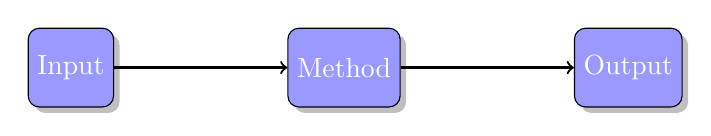
\begin{tikzpicture}[node distance=1.5cm]
        \node[component, anchor=center] (input) {Input};
        \node[component, anchor=center, right=2.2cm of input] (method) {Method};
        \node[component, anchor=center, right=2.2cm of method] (output) {Output};

        \draw[arrow] (input) -- (method);
        \draw[arrow] (method) -- (output);
    \end{tikzpicture}
    \caption{Example overview diagram. Replace with a figure that matches your report.}\label{fig:system_overview}
\end{figure}

\subsection{Organization}\label{sec:organization}

The rest of this report is organized as follows.\pref{sec:background} covers background and definitions.\pref{sec:methods} describes the methodology and core algorithm.\pref{sec:experiments} documents the experimental setup.\pref{sec:results} presents the results.\pref{sec:discussion} discusses limitations and implications.\pref{sec:conclusion} concludes the report. Additional details can be placed in\pref{app:additional_details}.


%!TeX root=../main.tex
% -----------------------------------------------------------------------------
% sections/background.tex
% Purpose: Background, notation, definitions, and related work.
%
% Keep this section concise: define only what is needed to understand the rest
% of the report. Move long derivations or extended proofs to the appendix.
% -----------------------------------------------------------------------------

\section{Background and Preliminaries}\label{sec:background}


\subsection{Notation (Example Table)}\label{sec:notation}

\pref{tab:notation} shows an example notation table. Replace the symbols and descriptions with those relevant to your report.

\begin{table}[t!]
    \centering
    \caption{Example notation table.}\label{tab:notation}
    \begin{threeparttable}
        \begin{tabular}{ll}
            \toprule
            Symbol & Meaning \\
            \midrule
            $n$ & Number of samples \\
            $d$ & Feature dimension \\
            $x_i \in \mathbb{R}^d$ & Input feature vector \\
            $y_i$ & Target / label \\
            $\theta$ & Model parameters \\
            \bottomrule
        \end{tabular}
    \end{threeparttable}
\end{table}

\subsection{Definitions and Theorems (Examples)}\label{sec:definitions}

\begin{definition}[Example Definition]\label{def:technical_report}
A \emph{technical report} is a document that describes a technical problem, the adopted approach, and supporting evidence (e.g., experiments, proofs, or analyses) in a reproducible way.
\end{definition}

We will refer back to \pref{def:technical_report} to illustrate cross-referencing in the template.

\begin{theorem}[Example Theorem]\label{theorem:amgm}
For any real numbers $a$ and $b$, we have $a^2 + b^2 \ge 2ab$.
\end{theorem}

\begin{proof}
The claim follows from the fact that $(a-b)^2 \ge 0$, which expands to $a^2 + b^2 - 2ab \ge 0$.
\end{proof}

\subsection{Example Equation}\label{sec:example_equation}

Use numbered equations for results that you will reference. For example, a standard regularized least-squares objective is:
\begin{equation}
\min_{\theta}\quad
\mathcal{L}(\theta)
=
\frac{1}{n}\sum_{i=1}^{n}\big\|f_{\theta}(x_i) - y_i\big\|_2^2
\;+\;
\lambda\|\theta\|_2^2,
\label{eq:least_squares}
\end{equation}
where $\lambda \ge 0$ controls the amount of regularization.

\subsection{Related Work (Placeholder)}\label{sec:related_work}


%!TeX root=../main.tex
% -----------------------------------------------------------------------------
% sections/methods.tex
% Purpose: Describe the methodology used in the report.
%
% Recommended contents:
% - High-level overview / design rationale
% - Formal problem definition (if not already in background)
% - Core algorithm(s) with pseudo-code
% - Complexity / resource analysis
% - Implementation details that affect reproducibility
% -----------------------------------------------------------------------------

\section{Methods}
\label{sec:methods}


\subsection{Approach Overview}
\label{sec:approach_overview}

At a high level, the method takes input data $D$, applies a sequence of processing steps, and produces an output artifact (e.g., a model, a set of results, or a system). Refer back to \pref{fig:system_overview} for the placeholder overview diagram.

\subsection{Core Objective (Example Equation)}
\label{sec:objective}

If your method can be described as an optimization problem, write the objective explicitly and reference it later. For example:
\begin{equation}
\min_{\theta}\quad
\mathcal{J}(\theta) = \mathcal{L}(\theta) + \alpha \mathcal{R}(\theta),
\label{eq:generic_objective}
\end{equation}
where $\mathcal{L}$ is a data-fit term, $\mathcal{R}$ is a regularizer, and $\alpha \ge 0$ balances the two.

\subsection{Algorithm (Example Pseudocode)}
\label{sec:algorithm}

\pref{alg:training_loop} shows a minimal example using \texttt{algorithm2e}. Replace it with your actual algorithm.

\begin{algorithm}[t!]
    \DontPrintSemicolon
    \KwIn{Dataset $D=\{(x_i,y_i)\}_{i=1}^{n}$, hyperparameters $\eta$}
    \KwOut{Trained parameters $\theta$}

    Initialize $\theta$ (e.g., randomly)\;
    \For{$t \gets 1$ \KwTo $T$}{
        Sample a minibatch $B \subseteq D$\;
        Compute gradient $g \gets \nabla_{\theta}\mathcal{J}(\theta; B)$\;
        Update $\theta \gets \theta - \eta g$\;
    }
    \Return{$\theta$}\;
    \caption{Example training loop.}
    \label{alg:training_loop}
\end{algorithm}

\subsection{Complexity and Resources (Placeholder)}
\label{sec:complexity}


%!TeX root=../main.tex
% -----------------------------------------------------------------------------
% sections/experiments.tex
% Purpose: Experimental setup and evaluation protocol.
%
% Recommended contents:
% - Datasets / benchmarks
% - Baselines
% - Metrics
% - Hardware / software environment
% - Reproducibility details (seeds, versions, configs)
% -----------------------------------------------------------------------------

\section{Experiments}\label{sec:experiments}


\subsection{Setup}\label{sec:experimental_setup}

\begin{itemize}
    \item Hardware.
    \item Software.
    \item Randomness.
\end{itemize}

\subsection{Datasets / Benchmarks (Example Table)}\label{sec:datasets}

\begin{table}[H]
    \centering
    \caption{Example dataset table (replace with your own).}\label{tab:datasets}
    \begin{tabular}{lrrl}
        \toprule
        Dataset & \#Samples & \#Features & Notes \\
        \midrule
        Dataset-A & 10{,}000 & 128 &  \\
        Dataset-B & 50{,}000 & 256 &  \\
        \bottomrule
    \end{tabular}
\end{table}

\subsection{Metrics (Example Definition)}\label{sec:metrics}

For example, if you report mean squared error (MSE), define it explicitly:
\begin{equation}
\mathrm{MSE} = \frac{1}{n}\sum_{i=1}^{n}{(\hat{y}_i - y_i)}^2.
\label{eq:mse}
\end{equation}

\subsection{Baselines and Ablations}\label{sec:baselines}

\begin{itemize}
    \item Baseline 1.
    \item Baseline 2.
    \item Ablation A.
\end{itemize}

\subsection{Implementation Details}\label{sec:implementation_details}



%!TeX root=../main.tex
% -----------------------------------------------------------------------------
% sections/results.tex
% Purpose: Present results, plots, and key findings.
%
% Keep the narrative focused:
% - What was measured?
% - What are the key quantitative results?
% - What are the most important qualitative observations?
% -----------------------------------------------------------------------------

\section{Results}\label{sec:results}


\subsection{Main Results (Example Table)}\label{sec:main_results}

\begin{table}[H]
    \centering
    \caption{Example results table. Replace metrics and values with your own.}\label{tab:results}
    \begin{tabular}{lrr}
        \toprule
        Method & MSE $\downarrow$ & Runtime (s) $\downarrow$ \\
        \midrule
        Baseline & 0.123 & 12.4 \\
        Proposed & 0.101 & 13.1 \\
        \bottomrule
    \end{tabular}
\end{table}

\subsection{Trend Visualization (Example Plot)}\label{sec:trend_plot}

\pref{fig:learning_curves} is an example plot generated with \texttt{pgfplots}. Replace it with your actual figures.

\begin{figure}[H]
    \centering
    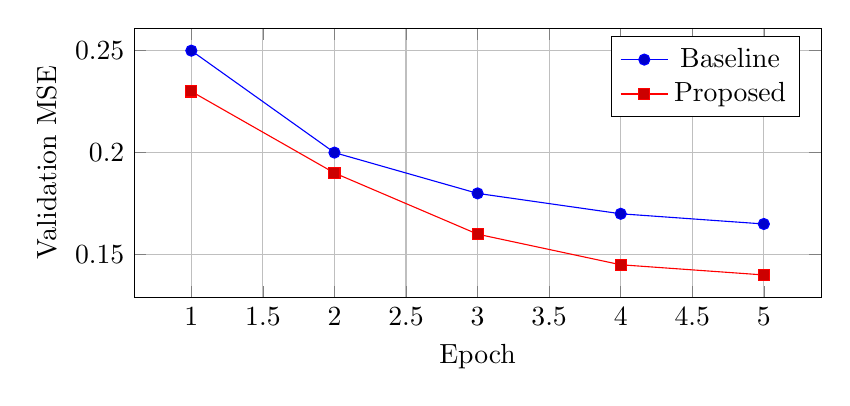
\begin{tikzpicture}
        \begin{axis}[
            width=0.85\linewidth,
            height=5cm,
            xlabel={Epoch},
            ylabel={Validation MSE},
            grid=both,
            legend pos=north east,
        ]
            \addplot+[mark=*] coordinates {
                (1,0.25) (2,0.20) (3,0.18) (4,0.17) (5,0.165)
            };
            \addlegendentry{Baseline}

            \addplot+[mark=square*] coordinates {
                (1,0.23) (2,0.19) (3,0.16) (4,0.145) (5,0.14)
            };
            \addlegendentry{Proposed}
        \end{axis}
    \end{tikzpicture}
    \caption{Example learning curves. Replace with your plot or a figure via \texttt{\string\includegraphics}.}\label{fig:learning_curves}
\end{figure}

\subsection{Key Takeaways}\label{sec:key_takeaways}

\begin{itemize}
    \item Finding 1.
    \item Finding 2.
    \item Finding 3.
\end{itemize}


%!TeX root=../main.tex
% -----------------------------------------------------------------------------
% sections/discussion.tex
% Purpose: Discuss implications, limitations, and future work.
% -----------------------------------------------------------------------------

\section{Discussion}\label{sec:discussion}


\subsection{Interpretation}\label{sec:interpretation}


\subsection{Limitations}\label{sec:limitations}

\begin{itemize}
    \item Limitation 1.
    \item Limitation 2.
    \item Limitation 3.
\end{itemize}

\subsection{Threats to Validity}\label{sec:threats_to_validity}


\subsection{Future Work}\label{sec:future_work}

\begin{itemize}
    \item Future work item 1.
    \item Future work item 2.
\end{itemize}


%!TeX root=../main.tex
% -----------------------------------------------------------------------------
% sections/conclusion.tex
% Purpose: Conclude the report.
%
% Recommended contents:
% - Short recap of the problem and contributions
% - Summary of main results
% - Practical implications (if any)
% - One or two clear next steps
% -----------------------------------------------------------------------------

\section{Conclusion}
\label{sec:conclusion}


In this template, we demonstrated a typical technical-report structure with examples of cross-references (\pref{sec:background}), equations (\pref{eq:least_squares}), algorithms (\pref{alg:training_loop}), tables (\pref{tab:results}), and figures (\pref{fig:learning_curves}).





\section*{Acknowledgment}
[Optional.] Acknowledge funding, collaborators, reviewers, and other support.

\bibliographystyle{plainnat}
\bibliography{references/references}

\appendix
\newpage
%!TeX root=../main.tex
% -----------------------------------------------------------------------------
% sections/appendix.tex
% Purpose: Put long proofs, derivations, extended tables, or extra figures here.
% -----------------------------------------------------------------------------

\section{Additional Details}
\label{app:additional_details}


\subsection{Extended Results (Example Table)}
\label{app:extended_results}

\begin{table}[t!]
    \centering
    \caption{Example appendix table.}
    \label{tab:appendix_example}
    \begin{tabular}{lrr}
        \toprule
        Setting & Metric-1 & Metric-2 \\
        \midrule
        Variant A & 0.42 & 1.7 \\
        Variant B & 0.39 & 1.9 \\
        \bottomrule
    \end{tabular}
\end{table}

\subsection{Extra Notes}
\label{app:extra_notes}



\end{document}
